\section{trace.c}
Trong hệ điều hành xv6, mỗi lời gọi hệ thống hay còn được gọi
là system call thì đều được định danh duy nhất bởi một số 
nguyên dương, bắt đầu từ 
\code{SYS\_fork = 1} đến \code{SYS\_close = 21} trong tệp tiêu 
đề \code{kernel/syscall.h}, đại diện cho $21$ system call 
cơ bản nhất được định nghĩa \cite{hcmus_os_lab2,xv6book}. Để tích hợp tính năng theo dõi tiến 
trình hay còn gọi là \texttt{trace}, ta cần thiết lập thêm mã định 
danh \code{SYS\_trace = 22}. Số hiệu này đóng một vai trò kép trong 
kiến trúc hệ thống: vừa là chỉ số tra cứu con trỏ hàm xử 
lý trong bảng điều phối \code{syscalls[]}, vừa xác định vị 
trí bit thứ $N$ (\code{1 << N}) trong mặt nạ theo dõi 
(\code{trace\_mask}). Nhờ cơ chế bitmask, chương trình người
dùng có thể linh hoạt giám sát một hoặc nhiều syscall đồng 
thời chỉ thông qua một số nguyên duy nhất, đồng thời cho phép 
kernel kiểm tra điều kiện kích hoạt bằng phép toán bitwise 
với độ phức tạp $O(1)$.

\subsection{Triển khai}
Để triển khai được tính năng \texttt{trace}, nhóm cần tạo
được một file \texttt{trace.c} ở trong thư mục \texttt{user/}.
Đây sẽ là nơi nhận lệnh \code{trace <mask\> <command\>}
để thực hiện quá trình theo dõi. Vì mỗi lệnh \texttt{trace} đều phải nhận 
vào một mặt nạ, đại diện cho các system call đang được theo dõi
tại một thời điểm $t$ nào đó. Do đó, ta phải định nghĩa một số nguyên
để có thể lưu trữ điều này ở ngay trong chính \code{struct proc} tại
\texttt{kernel/proc.h}. Và khi user gọi \code{trace} thì \texttt{mask} 
sẽ được truyền như là số nguyên vào system call \texttt{trace(int)}. Từ
đó mà ở phía dưới, kernel sẽ dùng hàm \code{sys\_trace()} (do nhóm tự khai
báo) tại \texttt{kernel/sysproc.c} sử dụng \code{argint(0, \&mask)} để tiếp
nhận tham số này và lưu nó trực tiếp vào tiến trình hiện hành
(\code{myproc()->trace\_mask}).

Quá trình xử lý đơn giản chỉ cần ta chuyển đối số \code{<mask\>}
thành một số nguyên và truyền vào hàm \code{trace(int)} để thực hiện việc 
theo dõi. Tuy nhiên, ở trong đề bài có một yêu cầu đó là \texttt{trace}
sẽ bật theo dõi cho tiến trình gọi nó và bất kỳ tiến trình con nào mà 
nó phân nhánh sau đó, nhưng không được ảnh hưởng đến các quy trình 
khác \cite{hcmus_os_lab2}. Do đó, khi tạo ra một proc mới ở trong hàm
\code{allocproc(void)} thì ta cần đặt lại về $0$ để biểu thị cho việc là
\texttt{proc} hiện tại chưa được theo dõi. Tiếp theo đó là khi một tiến 
trình gọi tiến trình con thì chính tiến trình con phải được kế 
thừa toàn bộ thông tin về các system call đang theo dõi từ cha. Như vậy,
ta cần sao chép \code{trace\_mask} của cha và gán nó vào cho con. Nhờ đó,
toàn bộ các tiến trình con cháu phân nhánh sau này đều được theo dõi 
liên tục mà vẫn bảo đảm tính cô lập, không làm ảnh hưởng đến các tiến 
trình độc lập khác trong hệ thống.

\paragraph*{Bắt và In}: Sau khi mà ta đã triển khai xong được cơ chế
lưu trữ và kế thừa thì bước quan trọng tiếp theo đó chính là tiến hành
bắt được các thông tin của syscall và in nó ra màn hình hệ thống tại
hàm điều phối \code{syscall(void)} trong file \texttt{kernel/syscall.c}.
Vì mặc định trong hệ điều hành \texttt{xv6} thì các syscall chỉ được lưu
dưới dạng các con số, nhưng bài toán yêu cầu ta phải in ra màn hình được
tên của syscall, nên để thuận tiện cho việc truy xuất và tiết kiệm thời 
gian, thì nhóm khai báo một mảng chuỗi ký tự \code{syscall\_names[]} để
có thể in tên ra màn hình một cách nhanh chóng. Và mỗi khi một system call 
được gọi, thì sau khi mà \textbf{con trỏ hàm} tương ứng đã thực thi xong
thì trả về kết quả lên thanh ghi \code{p->trapframe->a0}, và từ đó thì 
hệ thống sẽ tiến hành kiểm tra xem bit thứ \code{num} của system call 
đó có đang được bật trong \code{trace\_mask} hay không. Nếu bật thì kernel
sẽ in ra màn hình thông tin truy vết tương ứng theo đề bài yêu cầu đó
là: \texttt{<pid>: syscall <name> -> <return\_val>}. 

\subsection{Kiểm thử}
Sau khi hoàn tất quá trình triển khai và xử lý lời gọi hệ thống \texttt{trace}, nhóm tiến hành xây dựng các kịch bản kiểm thử nhằm đánh giá toàn diện tính đúng đắn của giải pháp. Bộ kiểm thử bao phủ từ các chức năng cơ bản, trường hợp biên, tính kế thừa phân nhánh cho đến khả năng xử lý lỗi hệ thống và tham số đầu vào (Bảng~\ref{tab:trace_testcases}).

\begin{table}[htbp]
    \centering
    \small
    \renewcommand{\arraystretch}{1.3}
    \begin{tabularx}{\textwidth}{p{0.41\textwidth} X}
        \toprule
        \textbf{Lệnh kiểm thử} & \textbf{Mục đích kiểm tra} \\
        \midrule
        \texttt{trace 32 grep hello README} 
            & Theo dõi duy nhất một system call (\texttt{SYS\_read = 5}, mặt nạ $1 \ll 5 = 32$). Hệ thống chỉ in các lời gọi \texttt{read}. \\
        \texttt{trace 32896 grep hello README} 
            & Theo dõi kết hợp \texttt{SYS\_exec} (7) và \texttt{SYS\_open} (15) với mặt nạ $(1 \ll 7) \mid (1 \ll 15) = 32896$. \\
        \texttt{trace 2147483647 grep hello README} 
            & Theo dõi toàn bộ các system call ($2^{31} - 1$, bật tất cả 31 bit đầu). \\
        \texttt{grep hello README} 
            & Chạy lệnh trực tiếp từ shell mà không qua \texttt{trace}. Xác nhận không có dòng vết nào bị rò rỉ (tính cô lập). \\
        \texttt{trace 0 grep hello README} 
            & Trường hợp biên với mặt nạ bằng 0. Lệnh vẫn chạy bình thường nhưng kernel không xuất bất kỳ log theo dõi nào. \\
        \texttt{trace 2 usertests forkforkfork} 
            & Theo dõi \texttt{SYS\_fork} (mặt nạ $1 \ll 1 = 2$) trên tiến trình sinh nhiều thế hệ con cháu để kiểm tra tính kế thừa. \\
        \texttt{trace 32896 grep hello no\_file} 
            & Cố tình truy xuất tệp không tồn tại để kiểm tra khả năng bắt lỗi và xuất thông báo từ hệ thống. \\
        \texttt{trace abc grep hello README} 
            & Kiểm tra xử lý lỗi người dùng khi nhập mặt nạ không phải chữ số. Chương trình từ chối thực thi và in hướng dẫn. \\
        \bottomrule
    \end{tabularx}
    \caption{Các kịch bản kiểm thử tính năng theo dõi system call}
    \label{tab:trace_testcases}
\end{table}

Kết quả thực nghiệm trên môi trường giả lập QEMU (Hình~\ref{fig:trace_results} và Hình~\ref{fig:trace_edge}) chứng minh toàn bộ các trường hợp đều hoạt động chính xác theo đặc tả của đề bài:
\begin{itemize}[noitemsep, topsep=2pt]
    \item \textbf{Theo dõi cơ bản và cô lập (Hình~\ref{fig:trace_results}):} Hệ thống lọc chính xác từng system call theo bitmask (như \texttt{read} ở Hình~\ref{fig:trace_32}, \texttt{exec} và \texttt{open} ở Hình~\ref{fig:trace_32896}, hoặc toàn bộ ở Hình~\ref{fig:trace_all}). Đồng thời, môi trường ngoài shell hoàn toàn không bị ảnh hưởng (Hình~\ref{fig:trace_none} và Hình~\ref{fig:trace_0}).
    \item \textbf{Kế thừa đa thế hệ (Hình~\ref{fig:trace_fork}):} Khi thực thi bài kiểm thử \texttt{forkforkfork}, các tiến trình con cháu liên tục kế thừa việc theo dõi \texttt{SYS\_fork} với các PID tăng dần ($146, 147, \dots$) cho đến khi bảng tiến trình đầy và trả về mã \texttt{-1}, kết thúc với \texttt{ALL TESTS PASSED}.
    \item \textbf{Xử lý ngoại lệ và tham số lỗi (Hình~\ref{fig:trace_edge}):} Khi gọi tệp không tồn tại (Hình~\ref{fig:trace_nofile}) hoặc truyền mặt nạ sai định dạng (Hình~\ref{fig:trace_invalid}), chương trình bắt lỗi chính xác và thông báo ra màn hình mà không làm sập hệ điều hành.
\end{itemize}

\begin{figure}[H]
    \centering
    \begin{subfigure}[b]{0.48\textwidth}
        \centering
        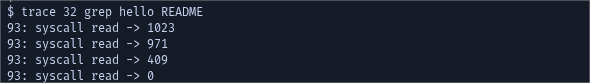
\includegraphics[width=\linewidth]{images/trace_32.png}
        \caption{Theo dõi \texttt{SYS\_read} (mask = 32)}
        \label{fig:trace_32}
    \end{subfigure}
    \hfill
    \begin{subfigure}[b]{0.48\textwidth}
        \centering
        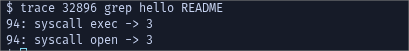
\includegraphics[width=\linewidth]{images/trace_32896.png}
        \caption{Theo dõi \texttt{exec} và \texttt{open} (mask = 32896)}
        \label{fig:trace_32896}
    \end{subfigure}
    
    \vspace{0.3cm}
    \begin{subfigure}[b]{0.48\textwidth}
        \centering
        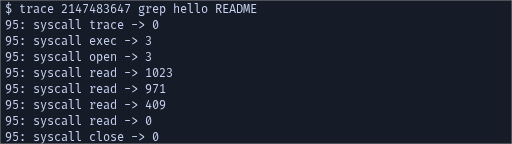
\includegraphics[width=\linewidth]{images/trace_all.png}
        \caption{Theo dõi toàn bộ syscall (mask = 2147483647)}
        \label{fig:trace_all}
    \end{subfigure}
    \hfill
    \begin{subfigure}[b]{0.48\textwidth}
        \centering
        
\includegraphics[width=\linewidth]{images/trace_none.png}
        \caption{Chạy trực tiếp ngoài shell (không qua trace)}
        \label{fig:trace_none}
        
        \vspace{0.3cm}
        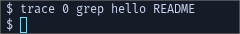
\includegraphics[width=\linewidth]{images/trace_0.png}
        \caption{Mặt nạ rỗng (mask = 0)}
        \label{fig:trace_0}
    \end{subfigure}
    \caption{Ảnh chụp kết quả kiểm thử các kịch bản theo dõi cơ bản và tính cô lập}
    \label{fig:trace_results}
\end{figure}

\begin{figure}[H]
    \centering
    \begin{subfigure}[b]{0.42\textwidth}
        \centering
        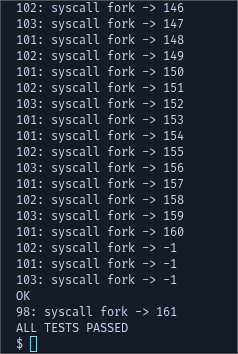
\includegraphics[width=0.88\linewidth]{images/trace_fork.png}
        \caption{Kế thừa qua phân nhánh (\texttt{forkforkfork})}
        \label{fig:trace_fork}
    \end{subfigure}
    \hfill
    \begin{minipage}[b]{0.54\textwidth}
        \begin{subfigure}[b]{\linewidth}
            \centering
            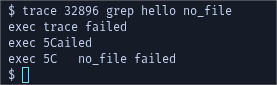
\includegraphics[width=0.85\linewidth]{images/trace_nofile.png}
            \caption{Truy xuất tệp không tồn tại}
            \label{fig:trace_nofile}
        \end{subfigure}
        
        \vspace{0.4cm}
        \begin{subfigure}[b]{\linewidth}
            \centering
            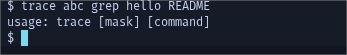
\includegraphics[width=0.85\linewidth]{images/trace_invalid.png}
            \caption{Nhập sai cú pháp tham số (\texttt{mask = abc})}
            \label{fig:trace_invalid}
        \end{subfigure}
    \end{minipage}
    \caption{Ảnh chụp kết quả kiểm thử tính kế thừa tiến trình và xử lý ngoại lệ}
    \label{fig:trace_edge}
\end{figure}
